\documentclass[border=4pt]{standalone}
\usepackage{tikz}
\usetikzlibrary{arrows.meta,positioning,calc,fit,backgrounds,patterns,shapes.geometric}
\usepackage{amsmath,amssymb}
\usepackage{mathptmx}
\definecolor{lost}{HTML}{C2362D}
\definecolor{kept}{HTML}{17875A}
\definecolor{evid}{HTML}{3056D3}
\definecolor{ink}{HTML}{1D1D1F}
\definecolor{muted}{HTML}{6E6E73}
\tikzset{
  box/.style={draw=ink!70, rounded corners=2pt, align=center, fill=white, inner sep=4pt, font=\footnotesize},
  arr/.style={-{Stealth[length=2mm]}, draw=ink!70, line width=0.6pt},
  grp/.style={draw=muted!60, dashed, rounded corners=4pt, inner sep=7pt},
  lossbox/.style={draw=lost!80, fill=lost!6, text=lost!85!black, rounded corners=2pt, align=left, font=\footnotesize, inner sep=4pt},
  fixbox/.style={draw=kept!80, fill=kept!7, text=kept!65!black, rounded corners=2pt, align=left, font=\footnotesize, inner sep=4pt},
  dec/.style={diamond, aspect=2.2, draw=ink!70, fill=evid!6, align=center, font=\footnotesize, inner sep=1.5pt},
  lbl/.style={font=\footnotesize\bfseries, text=ink},
}

\begin{document}
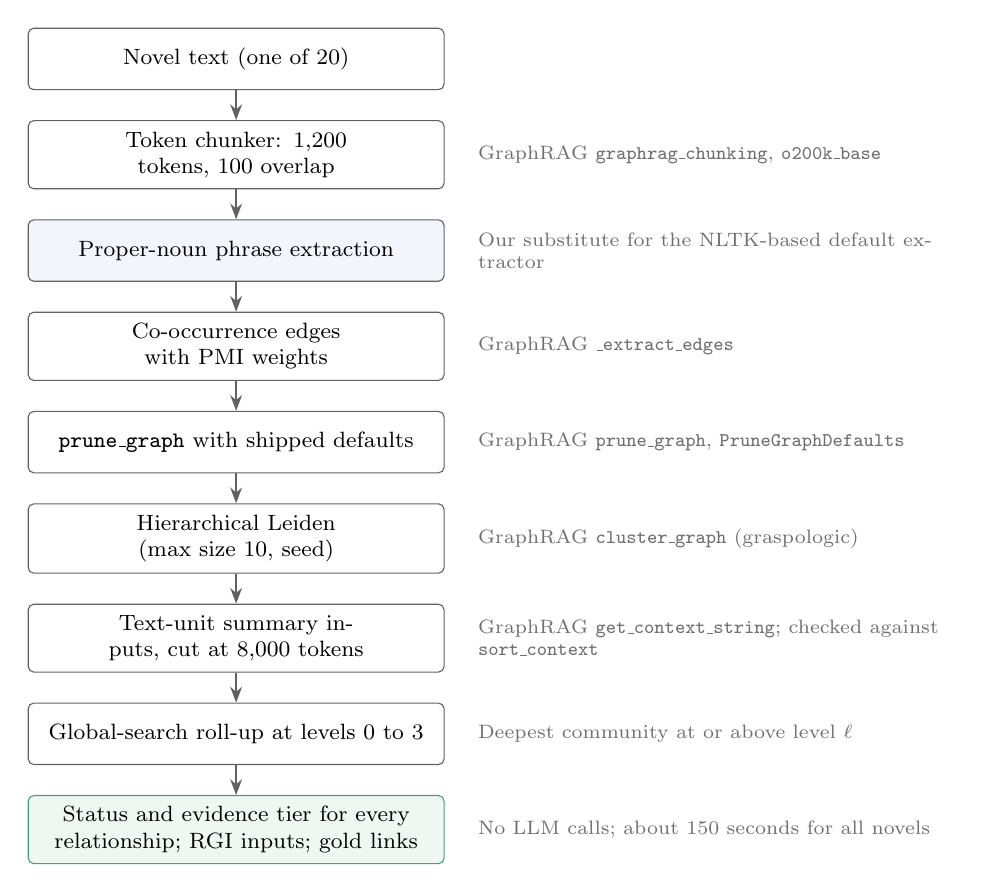
\begin{tikzpicture}[node distance=0.38cm]
\tikzset{st/.style={box, minimum width=5.2cm, minimum height=0.78cm, text width=5.0cm}, note/.style={font=\scriptsize, text=muted, align=left, text width=6.2cm, anchor=west}}
\node[st] (n1) {Novel text (one of 20)};
\node[st, below=of n1] (n2) {Token chunker: 1,200 tokens, 100 overlap};
\node[st, below=of n2, fill=evid!6] (n3) {Proper-noun phrase extraction};
\node[st, below=of n3] (n4) {Co-occurrence edges with PMI weights};
\node[st, below=of n4] (n5) {\texttt{prune\_graph} with shipped defaults};
\node[st, below=of n5] (n6) {Hierarchical Leiden (max size 10, seed)};
\node[st, below=of n6] (n7) {Text-unit summary inputs, cut at 8,000 tokens};
\node[st, below=of n7] (n8) {Global-search roll-up at levels 0 to 3};
\node[st, below=of n8, fill=kept!7, draw=kept!80] (n9) {Status and evidence tier for every relationship; RGI inputs; gold links};
\foreach \a/\b in {n1/n2,n2/n3,n3/n4,n4/n5,n5/n6,n6/n7,n7/n8,n8/n9} \draw[arr] (\a) -- (\b);
\node[note] at ($(n2.east)+(0.3,0)$) {GraphRAG \texttt{graphrag\_chunking}, \texttt{o200k\_base}};
\node[note] at ($(n3.east)+(0.3,0)$) {Our substitute for the NLTK-based default extractor};
\node[note] at ($(n4.east)+(0.3,0)$) {GraphRAG \texttt{\_extract\_edges}};
\node[note] at ($(n5.east)+(0.3,0)$) {GraphRAG \texttt{prune\_graph}, \texttt{PruneGraphDefaults}};
\node[note] at ($(n6.east)+(0.3,0)$) {GraphRAG \texttt{cluster\_graph} (graspologic)};
\node[note] at ($(n7.east)+(0.3,0)$) {GraphRAG \texttt{get\_context\_string}; checked against \texttt{sort\_context}};
\node[note] at ($(n8.east)+(0.3,0)$) {Deepest community at or above level $\ell$};
\node[note] at ($(n9.east)+(0.3,0)$) {No LLM calls; about 150 seconds for all novels};
\end{tikzpicture}
\end{document}
